\section{Question 1: How Does Distributional Shift Affect Performance?}
\label{sec:sampling_distributions}

%As alluded to in Section~\ref{sec:analysis_nonstationarity}, the choice of sampling distribution $\mu$ is an important design decision can have a large impact on performance. Indeed, it is not immediately clear which distribution is ideal for Q-learning. In this section, we hope to shed some light on this issue.

%\subsection{Technical Background}
% Off-policy data has been cited as one of the ``deadly triads'' for Q-learning~\citep{suttonrlbook}, which has potential to cause instabilities in learning. On-policy distributions~\citep{Tsitsiklis1997} and fixed behavior distributions~\citep{Sutton09a,Maei2010} have often been targeted for theoretical convergence analysis, and many works use importance sampling to correct for off-policyness~\citep{precup2001offpol, munos2016safe}
% However, to our knowledge, there is relatively little guidance which compares how different weighting distributions compare in terms of convergence rate and final solutions.

Off-policy RL methods applied to the offline RL problem would typically attempt to learn an optimal policy, even though the static dataset may not be generated from an optimal policy. As a result, one challenge that is expected to emerge is \emph{distributional shift} in many forms: abstractly, while these methods can only train the Q-function and the policy using state-action tuples generated by the behavioral policy, the policy will need to make correct predictions on states sampled from a different distribution, that it will encounter during a rollout at test time. In general, machine learning models are not robust when the distribution of inputs changes, indicating that distributional shift can be challenge for off-policy RL methods. Is distributional shift a challenge in offline RL?   

Indeed, theoretically, the effects of distributional shift have been quantified using the notion of a concentrability coefficient~\citep{munos2005erroravi}, a constant typically $\ggt 1$, which provides a worst-case error bound on the performance of an off-policy RL method due to distributional shift. To evaluate if this challenge persists empirically as well, we will analyze Q-learning methods for various choices of data distributions in this section. 

A crucial design decision we must make is to consider setups that do not confound distributional shift with access to limited data. Therefore, for our study, we provide the underlying algorithm oracle access to all state-action transitions in the MDP, but vary the \emph{distribution} over state-action pairs that these transitions are sampled according to.   
% ~\citep{NIPS2017_6913} suggests that when the state-distribution is fixed, the action distribution should be weighted by the optimal policy for residual Bellman errors. In deep RL, prioritized replay~\citep{Schaul2015}, and mixing replay buffer with on-policy data~\citep{hausknecht2016policy,zhang2018deeper} have been found to be effective. %We aim to empirically analyze multiple choices for weighting distributions to determine which are the most effective.

%\vspace{-10pt}
\subsection{What Are the Best Data Distributions Without Sampling Error?}
\label{subsec:dist_shift_exact}

% \begin{figure*}[ttt!]
% \begin{subfigure}{0.3\linewidth}
% \caption{\footnotesize \label{fig:distribution_shift_vs_returns} Average distribution shift across time for different data distributions, plotted against returns for a 256x256 model. We find that distribution shift does not have strong correlation with returns.}
% 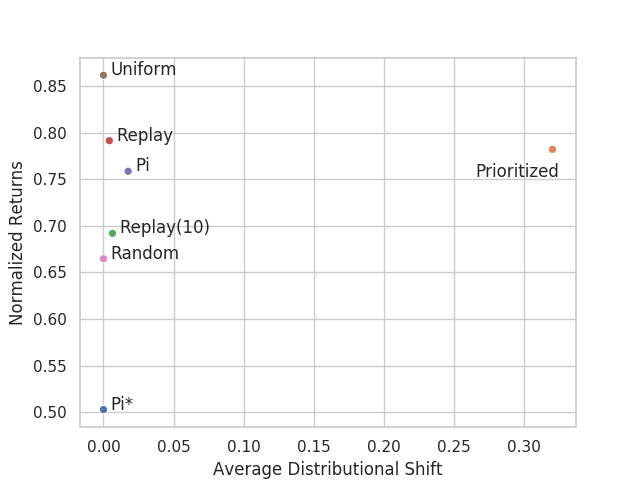
\includegraphics[width=0.99\columnwidth]{chapters/diagnosing_q/images/returns_vs_shift}
% % generated by plot_distribution_shift.py
% % data_dir = east1//2019-02-12-exact-weighting-distr-shift
% \vspace{-0.2in}
% \end{subfigure}
% ~\vline~
% \begin{subfigure}{0.3\linewidth}
% \caption{\footnotesize \label{fig:weighting_schemes} Weighting distribution versus architecture in Exact-FQI. Replay(s, a) consistently provides the highest performance. Note that Adversarial Feature Matching is comparable to Replay(s, a), but surprisingly better for small networks. }
% 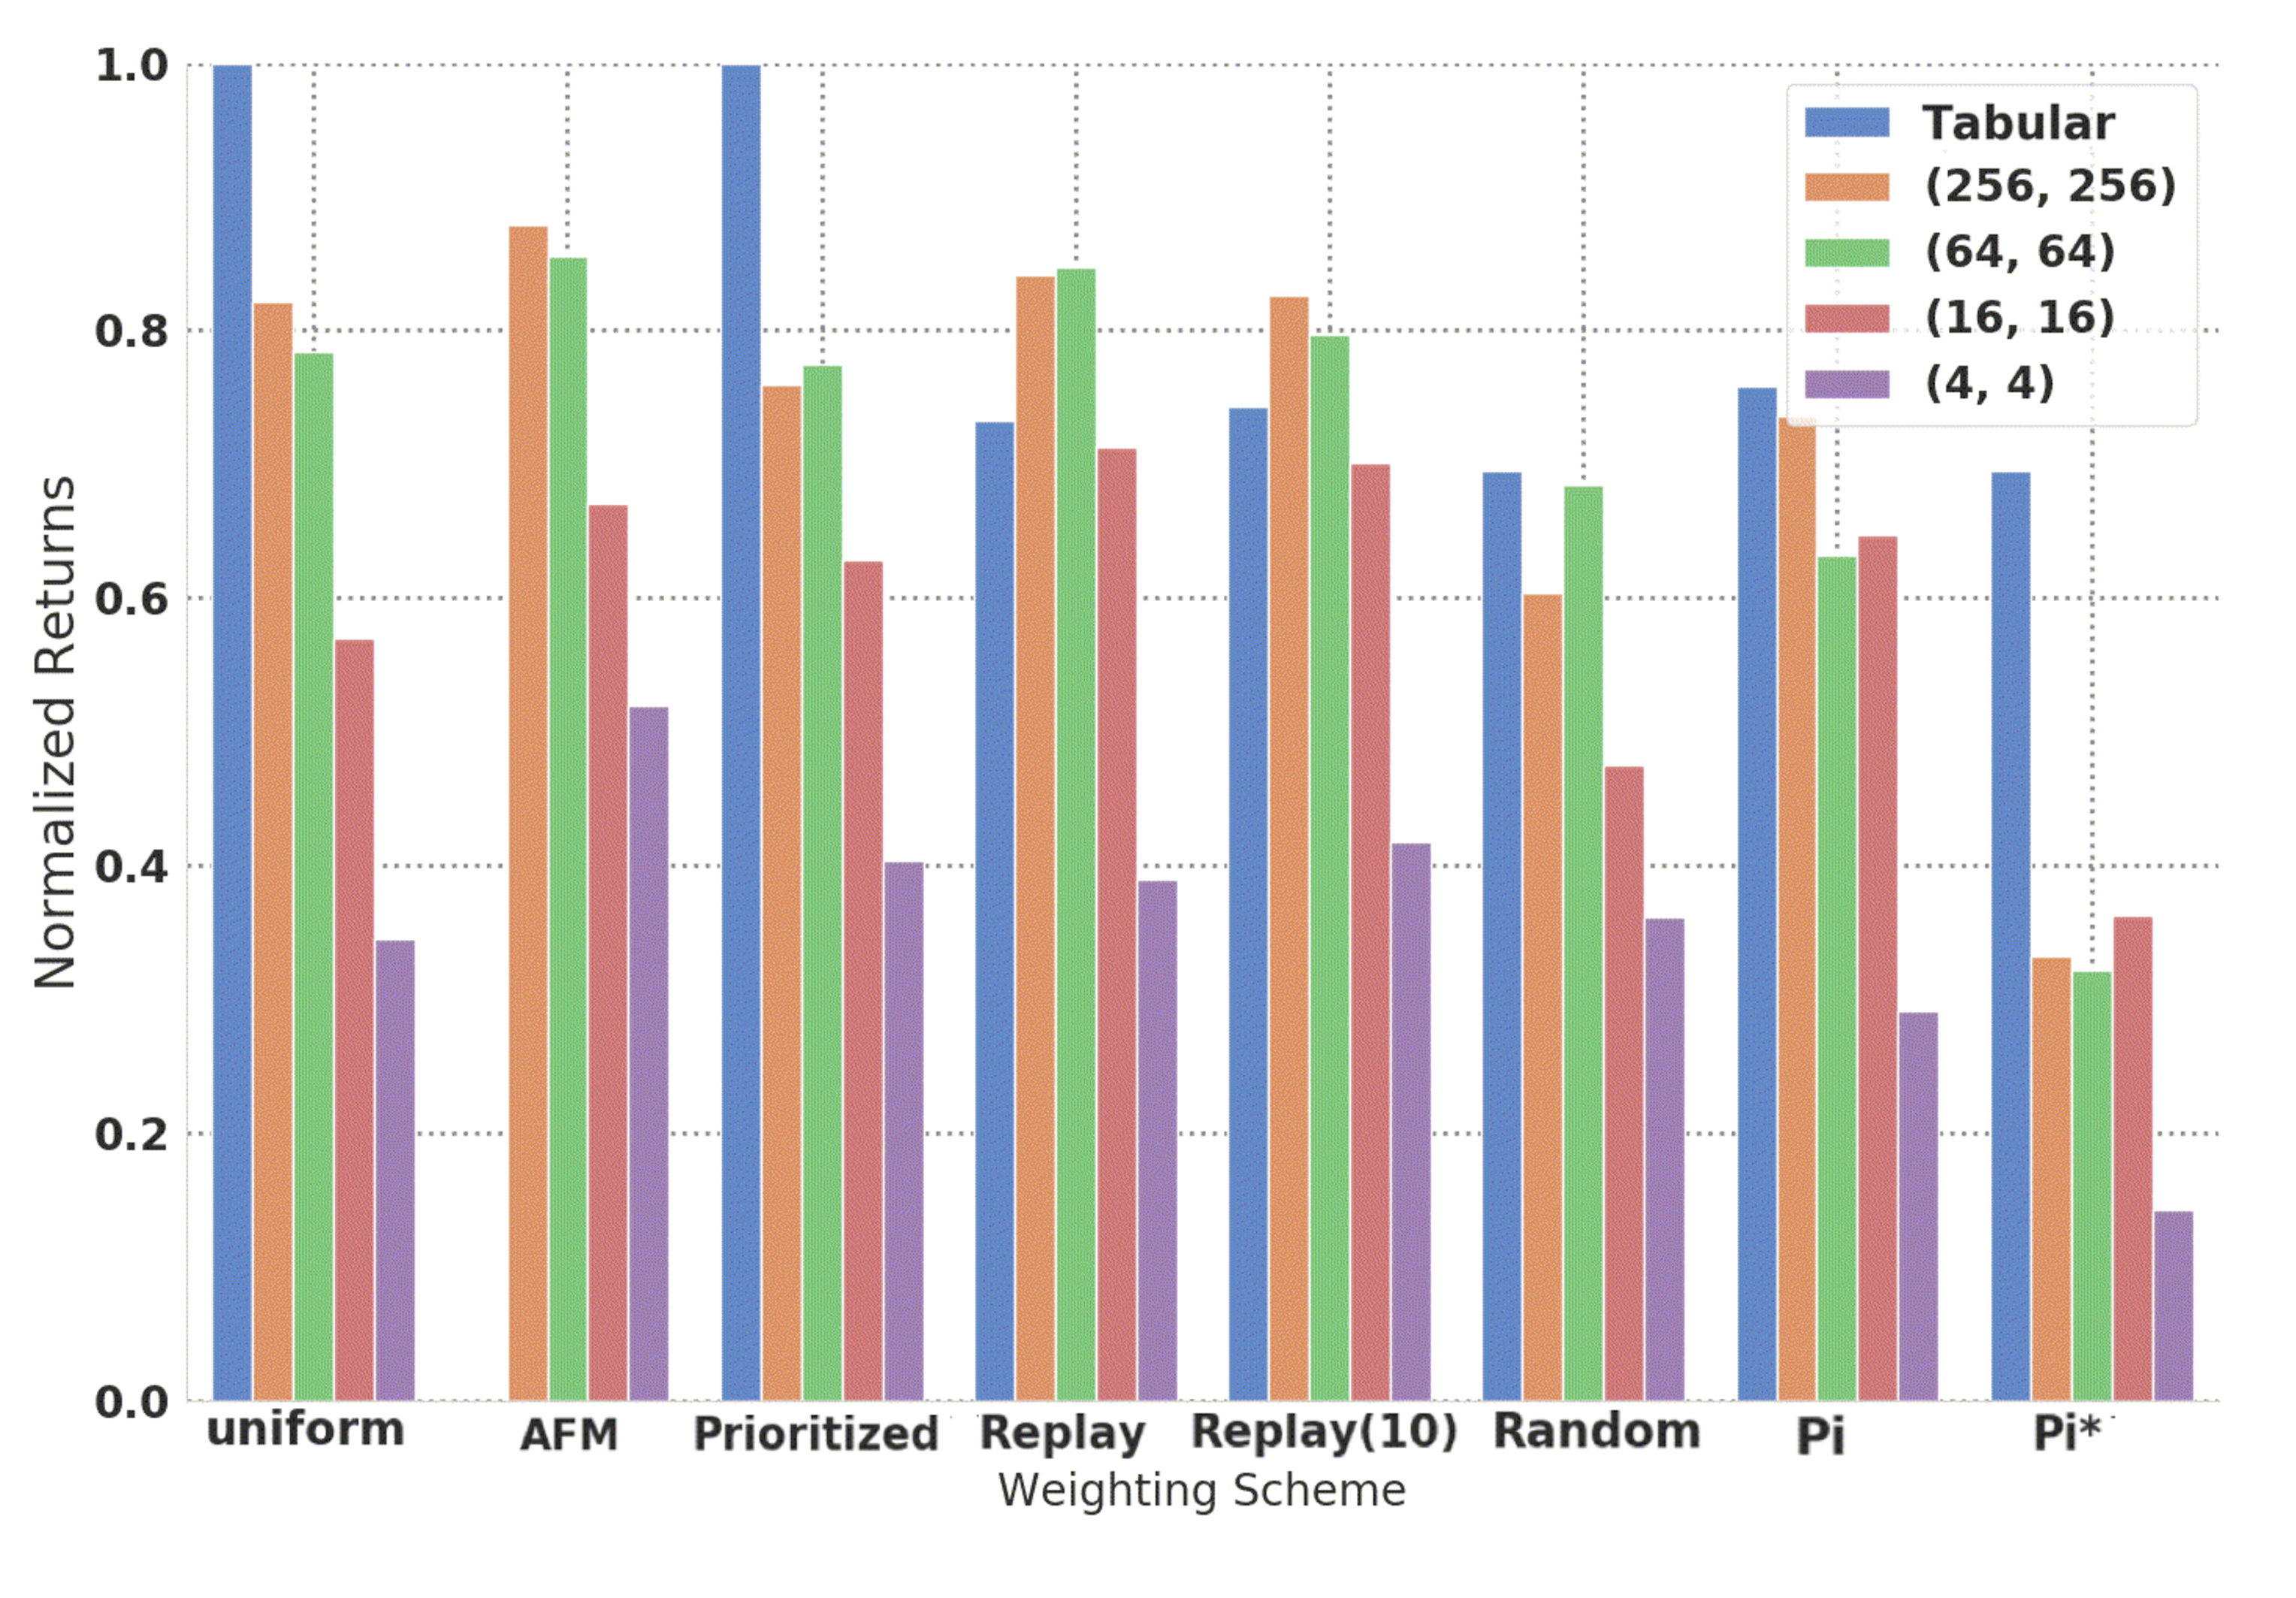
\includegraphics[width=0.99\columnwidth]{chapters/diagnosing_q/images/exact_fqi_schemes.pdf}
% % generated by plot_exact_weighting.py
% % data_dir = east1//2019-01-18-newenv-exact-weighting
% \vspace{-0.3in}
% \end{subfigure}
% ~\vline~
% \begin{subfigure}{0.3\linewidth}
% \caption{\footnotesize \label{fig:weighting_entropy_vs_returns} Normalized returns plotted against normalized entropy for different weighting distributions. All experiments use Exact-FQI with a 256x256 network. We see a general trend that high-entropy distributions lead to greater performance.}
% 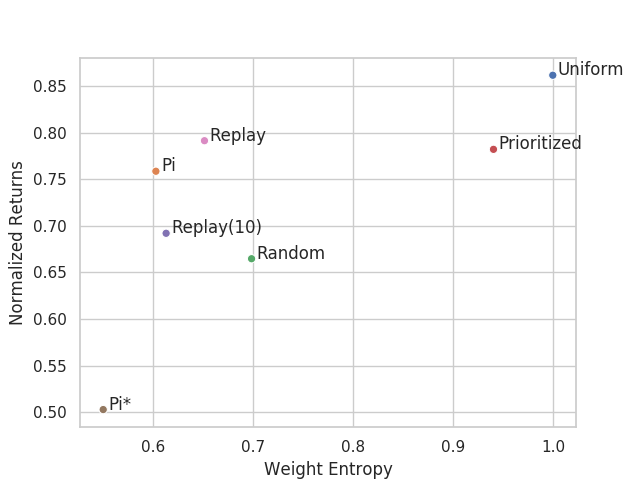
\includegraphics[width=0.99\columnwidth]{chapters/diagnosing_q/images/returns_vs_entropy}
% % generated by plot_distribution_shift.py
% % data_dir = east1//2019-02-12-exact-weighting-distr-shift
% \end{subfigure}
% \end{figure*}

\begin{wrapfigure}{r}{0.45\linewidth}
    \vspace{-0.2cm}
    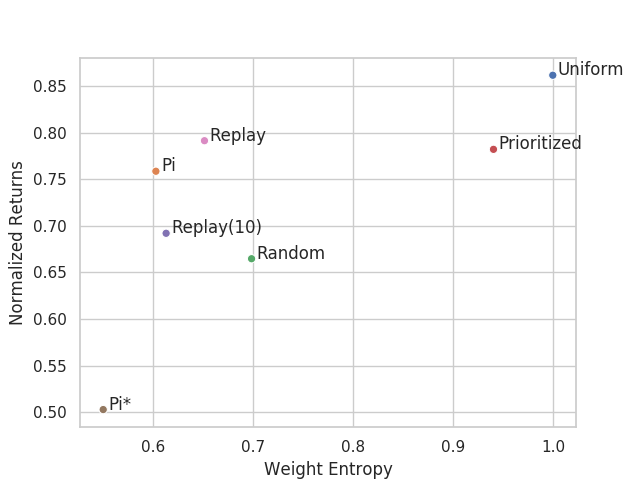
\includegraphics[width=0.99\linewidth]{chapters/diagnosing_q/images/returns_vs_entropy}
    \caption{\footnotesize \label{fig:weighting_entropy_vs_returns} Normalized returns plotted against normalized entropy for different weighting distributions. All experiments assume access to all state-action pairs with a 256x256 Q-network. We see a general trend that high-entropy distributions lead to greater performance, corroborating the uniformity hypothesis.}
    \vspace{-0.2cm}
    % generated by plot_distribution_shift.py
    % data_dir = east1//2019-02-12-exact-weighting-distr-shift
\end{wrapfigure}
We begin by studying the effect of data distributions when disentangled from sampling error. We run Q-learning with an ablation over various Q-function network architectures and data distributions and report our aggregate results in Fig.~\ref{fig:weighting_entropy_vs_returns}. $\text{Unif}(\bs, \mathbf{a})$, $\text{Replay}(\bs, \mathbf{a})$ (using a replay buffer consisting of data from a mixture of policies with different degrees of optimality), and $\text{Prioritized}(\bs, \mathbf{a})$ (weighting induced by prioritized experience replay~\citep{Schaul2016PrioritizedER}) consistently result in the highest returns across all architectures. On the other hand, relatively "narrow" data distributions, such as those induced the optimal policy ($\pi^*$) or only using a mixture of a few policies ($\text{Replay}(10)$) results in poor performance.
We believe that these results are in favor of the \textit{uniformity} hypothesis: intuitively, the best distributions spread weight across larger support of the state-action space, reducing the amount of possible distributional shift. On the other hand, less-uniform distributions such as the state-action distirbution induced by the optimal policy, present multiple avenues to deviate away from the offline data distribution, resulting in larger distributional shift.

\textbf{To summarize}, this indicates that narrow data distributions lead to worse performance compared to higher-entropy data distributions, indicating that distributional shift can have a significant impact on the performance of off-policy RL in the offline setting.
%These distributions generally result in the tightest contraction rates, and allow the Q-function to focus on high-error regions. 
%In the sampled setting, this observation motivates exploration algorithms that maximize state coverage (for example, ~\citet{hazan2018} solve an exploration objective which maximizes state-space entropy).
%However, note that in this particular experiment is distinct from exploration, as there is no sampling involved. 
%All states are observed, just with different weights, thus isolating the issue of distributions from the issue of sampling.

\iffalse

\subsection{Designing a Better Off-Policy Distribution: Adversarial Feature Matching}
\label{sec:afm}

In our final study, we attempt to design a better weighting distribution using insights from previous sections that can be integrated into deep RL methods. We refer to this method as adversarial feature-matching (AFM). We draw upon three specific insights outlined in previous analysis. First, the function approximator should be incentivized to maximize its ability to distinguish states to minimize function approximation bias (Section~\ref{sec:function_approx}). Second, the weighting distribution should emphasize areas where the Q-function incurs high Bellman error, to minimize the discrepancy between $\ltwonorm$ norm error and $\linfnorm$ norm error. Third, high-entropy weighting distributions tend to be higher performant. The first insight was also demonstrated in \cite{martha2018sparse} where enforcing sparsity in the Q-function was found to provide locality in the Q-function which prevented catastrophic interference and provided better values for bootstrapping.

We propose to model our problem as a minimax game, where the weighting distribution is a parameterized adversary $p_\phi(s, a)$ which tries to \emph{maximize} the Bellman error, while the Q-function ($Q_\theta(s, a)$) tries to minimize it. 
Note that in the unconstrained setting, this game is equivalent to minimizing the $\linfnorm$ norm error in its dual-norm representation. However, in practical settings where minimizing stochastic approximations of the $\linfnorm$ norm can be difficult for neural networks, it is crucial to introduce constraints to weaken the adversary. These constraints also make the adversary closer to the uniform distribution while allowing it to be sufficiently different at specific state-action pairs.

We use a feature matching constraint which enforces the expected feature vectors, $\mathbb{E}[\Phi(s)]$, under $p_\phi(s, a)$ to \emph{roughly} match the expected feature vector under uniform sampling from the replay buffer. We can express the output of a neural network Q-function as $Q_\theta(s, a) = w_{a}^T \Phi_\theta(s)$ or, in the continuous case, as $Q_\theta(s, a) = w^T \Phi_\theta(s, a)$,  where the feature vector $\Phi_\theta(s), \Phi_\theta(s, a)$ represent the the output of all but the final layer.
Intuitively, this constraint restricts the adversary to distributing probability mass among states that are perceptually similar to the Q-function. The objective is
\begin{multline*}
    \min_{\theta, w} \max_{\phi} \mathbb{E}_{p_\phi(s, a)} [(Q_{w, \theta} (s, a) - y(s, a))^2]\\
s.t.~~ \vert\vert \mathbb{E}_{p_\phi(s, a)}[\Phi(s)] - \frac{\sum_i \Phi(s_i)}{N} \vert\vert \leq \varepsilon
\end{multline*}
Note that $\Phi(s)$ is a function of $\theta$ but, while solving the maximization, $\theta$ is assumed to be a constant. This is equivalent to solving only the inner maximization with a constraint, and empirically provides better stability. Implementation details for AFM are provided in \textbf{Appendix \ref{app:adversarial}}. The $\frac{\sum_{i} \Phi(s_i)}{N}$ denotes an estimator for the true expectation under some sampling distribution, such as a uniform distribution over all states and actions (in exact FQI) or the replay buffer distribution. So, $\frac{\sum_{i} \Phi(s_i)}{N} \approx E_{p_{rb}}[\Phi]$ holds when using a replay buffer.

In tabular domains with Exact-FQI, we find that AFM performs at par with the top performing weighting distributions, such as $\text{Unif}(s, a)$ and \textit{better} than $\text{Prioritized}(s, a)$ (Fig.~\ref{fig:weighting_schemes}). This confirms that adaptive prioritization works better than Prioritized($s, a$). Another benefit of AFM is its robustness to function approximation and the performance gains in the case of small architectures (say, $(4, 4)$) are particularly noticeable. (Fig.~\ref{fig:weighting_schemes})

In tabular domains with Replay-FQI (Table~\ref{table:final}), we also compare AFM to prioritized replay (PER)~\citep{Schaul2015}, where AFM and PER perform similarly in terms of normalized returns. We also evaluate a variant of AFM (AFM+Sampling in Table~\ref{table:final}) which changes which samples instead of reweighting. We further evaluate AFM on MuJoCo tasks with the TD3 algorithm~\citep{pmlr-v80-fujimoto18a} and the entropy constrained SAC algorithm~\citep{Haarnoja18}. The results are presented in the appendix. We find AFM improving performance of the algorithm with three MuJoCo tasks (Ant, Hopper and Cheetah) and two algorithms (TD3 and SAC).

\begin{table}
    \centering
    \small{
    \begin{tabular}{|c|r|r|}
    \hline
    \textbf{Sampling distribution} & \textbf{Norm. Returns} & \textbf{Norm. Returns} \\
     & \textbf{(16, 16)} & \textbf{(64, 64)} \\
     \hline\hline
    None &  0.18 & 0.23 \\
    \hline
    Uniform(s, a) &  0.19 & 0.25 \\
    \hline
    $\pi(s, a)$ &  \textbf{0.45} & 0.39 \\
    \hline
    $\pi^*(s, a)$ & 0.30 & 0.21 \\
    \hline
    Prioritized(s, a) & 0.17 & 0.33 \\
    \hline
    PER~\cite{Schaul2015} & 0.42 & \textbf{0.49}\\
    \hline
    \textbf{AFM} (Ours) & 0.41 & \textbf{0.48} \\
    \hline
    \textbf{AFM + Sampling} (Ours) & 0.43 & \textbf{0.51} \\
    \hline
     \end{tabular}}
    \caption{\label{table:final}Average Performance of various sampling distributions for (16, 16) and (64, 64) neural nets in the setting with replay buffers averaged across 5 random seeds. PER, our AFM and on-policy sampling perform roughly at par on benchmark tasks in expectation when using (16, 16) architectures. However, note that  $\pi(s,a)$ is generally computationally intractable.}
    \vspace{-0.2in}
    \vspace{-10pt}
\end{table}

\fi